%%%%%%%%%%%%%%%%%%%%%%%%%%%%%%%%%%%%%%%%%%%%%%%%%%%%%%%%%%%
% --------------------------------------------------------
% Rho
% LaTeX Template
% Version 1.0 (28/04/2024)
%
% Author: 
% Guillermo Jimenez (memo.notess1@gmail.com)
% 
% License:
% Creative Commons CC BY 4.0
% --------------------------------------------------------

\documentclass[9pt,a4paper,twoside]{rho}
\usepackage[english]{babel}

\usepackage{rhoenvs}

%----------------------------------------------------------
% TITLE
%----------------------------------------------------------

\title{Rapport de stage de M1 : déconvolution parcimonieuse pour la maintenance prédictive de câbles haute-tension}

%----------------------------------------------------------
% AUTHORS AND AFFILIATIONS
%----------------------------------------------------------

\author[1]{Yanis Gomes}


%----------------------------------------------------------

\affil[1]{Ecole Normale Supérieure de Paris-Saclay}


%----------------------------------------------------------
% DATES
%----------------------------------------------------------

\dates{Août 20, 2024}

%----------------------------------------------------------
% FOOTER INFORMATION
%----------------------------------------------------------

%\smalltitle{Rapport de stage de recherche au}
%\institution{Centre Borelli - ENS Paris-Saclay}

%----------------------------------------------------------
% ARTICLE INFORMATION
%----------------------------------------------------------

%\corres{Provide the corresponding author information and publisher here.}
\email{yanis.gomes@ens-paris-saclay.fr}
%\doi{\url{https://www.doi.org/exampledoi/XXXXXXXXXX}}
%
%
%\license{Rho LaTeX Class \ccLogo\ This document is licensed under Creative %Commons CC BY 4.0.}
%
%----------------------------------------------------------
% ABSTRACT
%----------------------------------------------------------

\begin{abstract}
    Ce rapport décrit l'amélioration d'un algorithme de codage convolutionnel parcimonieux pour la maintenance non-destructive des câbles à haute tension. 
    En utilisant la technique de fuite de flux magnétique pour détecter les défauts dans les câbles on arrive à reconstruire précisément les défauts réels des câbles haute-tension en les interprétant comme la superposition de motifs de défauts théoriques paramétriques.
    Nous avons exploré et amélioré les algorithmes classiques de détection de motifs, en se concentrant particulièrement sur la déconvolution de motifs superposés.
    Nous avons ainsi démontré que l'introduction d'une approche combinatoire et arborescente dans l'exploration atomique du dictionnaire convolutionnel a significativement renforcé les capacités de déconvolution sur les intervalles comportant des atomes superposés.
\end{abstract}
%----------------------------------------------------------

\keywords{Codage Convolutionnel Parcimonieux, Maintenance Prédictive, Câbles Haute-Tension, Fuite de Flux Magnétique, Dictionnaires Convolutionnels, Orthogonal Matching Pursuit}

%----------------------------------------------------------

\begin{document}
	
\maketitle
\thispagestyle{firststyle}
% \tableofcontents

%----------------------------------------------------------

%% REMERCIEMENTS

\section{Introduction}

\subsection{Remerciements}
Je tiens à remercier sincèrement mes encadrants de stage, Charles Truong et Laurent Oudre, pour leur guidance précieuse et leur soutien durant ce stage de recherche de M1. Leur expertise et leurs conseils ont grandement contribué à mon apprentissage et à ma progression académique.

\subsection{Le Centre Borelli}
Le Centre Borelli, officiellement connu sous le nom d'Unité Mixte de Recherche (UMR 9010), réunit des experts en mathématiques, informatique et neurosciences. 
Ces chercheurs travaillent activement aux interfaces avec le domaine biomédical et le transfert industriel, illustrant l'engagement du centre dans des collaborations transdisciplinaires poussées. 
Implanté sur plusieurs sites, dont l’ENS Paris-Saclay et l’Université Paris Cité, le centre se distingue par son approche interdisciplinaire qui embrasse la modélisation, la simulation et le traitement de données complexes.

La démarche scientifique du Centre Borelli est caractérisée par une intégration profonde de la théorie mathématique avec des applications pratiques, y compris le développement de technologies numériques et de méthodes cliniques. 
Cela se manifeste par un fort engagement dans la science reproductible et une forte interaction avec les phénomènes réels à travers des observations sur le terrain et l'expertise transdisciplinaire.

Les axes de recherche du centre sont variés, englobant depuis le traitement des images et des signaux jusqu'à la modélisation de phénomènes complexes dans les sciences physiques, naturelles et biologiques. 
L'équipe s'investit également dans les neurosciences comportementales, apportant des perspectives quantitatives sur le comportement humain et animal en situation normale ou pathologique.

\begin{figure}[H]
    \centering
    
\includegraphics[width=0.3\linewidth]{images/borelli.png}
    \caption{Logo du Centre Borelli, un laboratoire interdisciplinaire de recherche en mathématiques, informatique et neurosciences}
    \label{fig:lab2}
\end{figure}

\subsection{Contexte}

Le stage s'inscrit dans le cadre de la chaire PHLAMES portant sur la Physique des Lignes Aériennes Modélisations, Expériences et Simulations, une collaboration entre l'ENS Paris-Saclay et RTE le Réseau de Transport d'Electricité. Cette initiative vise à adresser des défis techniques et scientifiques liés au transport d'électricité haute tension.
Un défi majeur se pose : la majorité des lignes haute tension en France ont été installées en même temps elles approchent donc de la fin de leur durée de vie simultanément.
Cette synchronicité pose des problèmes logistiques et financiers significatifs, car le renouvellement simultané de ces infrastructures est à la fois coûteux et critique pour la pérennité du réseau électrique national et européen.

Face à ce défi, RTE se doit de planifier intelligemment le renouvellement des câbles haute tension pour maintenir la stabilité et la fiabilité du réseau.
L'approche non-destructive est donc essentielle dans la gestion du transport d'électricité à grande échelle, où il est crucial de minimiser les interruptions tout en optimisant les interventions.
Dans ce contexte, la technique de fuite de champ magnétique ou Magnetic Flux Leakage (MLF) devient un outil incontournable \cite{broken_wire}. Cette méthode permet de détecter et d'analyser les défauts structurels des câbles sans les endommager.

\begin{figure}[H]
    \centering
    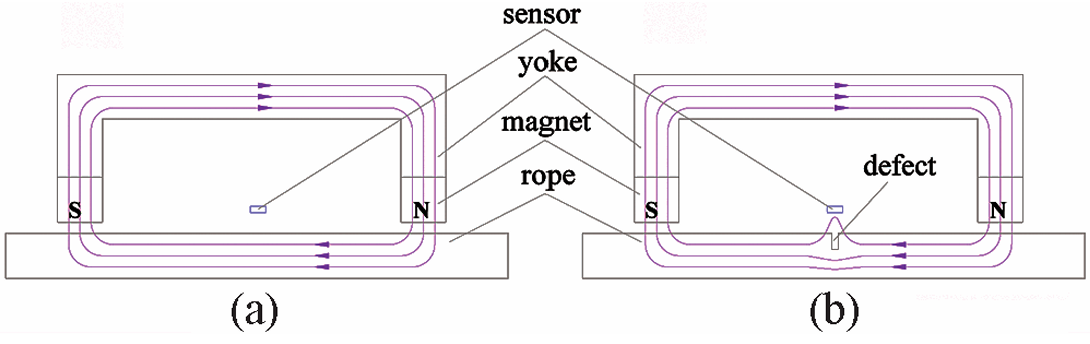
\includegraphics[width=1\linewidth]{images/magnetic_flux_leakage.png}
    \caption{Schéma de principe de la détection de fuite de champ magnétique : (a) Sans défaut, (b) Avec défaut}
    \label{fig:mfl}
\end{figure}

La technique de Magnetic Flux Leakage (MFL) est aujourd'hui bien maîtrisée, tant sur le plan de la modélisation physique que de son application pratique, une machine capable de se déplacer le long d'un câble installé a été spécialement conçue à cette occasion.
Le défi principal réside donc dans le traitement des données collectées sur des câbles en conditions réelles. 

Ce stage au Centre Borelli s'inscrit dans la continuité de ces travaux, visant à améliorer les algorithmes de déconvolution parcimonieuse pour la maintenance prédictive des câbles haute tension.


\subsection{Problématique}

Pour établir une priorité dans le remplacement des câbles à haute tension, il est essentiel de mesurer précisément les défauts présents. 
Cela implique l'identification de la position et des paramètres des défauts en se basant sur un dictionnaire de motifs paramétriques théoriques issue de la modélisation physique des câbles haute-tension. 
Toutefois, les défauts réels résultent souvent d'une superposition de ces motifs théoriques, complexifiant ainsi leur détection et leur analyse.
Pour améliorer la maintenance prédictive et la gestion des ressources du réseau électrique, il est nécessaire d'arriver à une déconvolution efficace permettant d'expliquer la présence de motifs complexes dans les signaux à partir d'un dictionnaire de motifs théoriques élémentaires.
Notre étude repose donc sur la problématique clef :

\begin{center}
    \textbf{Comment peut-on améliorer les algorithmes de déconvolution parcimonieuse pour mieux identifier et caractériser les motifs superposés dans les défauts de câbles haute tension?}
\end{center}


\section{Préliminaires}

\subsection{Modélisation physique}

Comme dans \cite{broken_wire} et \cite{localized_defects_omp} le champ de fuite magnétique d'une surface en acier est modélisé par un modèle de dipôle magnétique.
Dans ce cadre, la composante radiale $H_r$ du champ magnétique à la position $x$ le long du câble est donnée par la formule de Zatsepin et Shcherbinin abrévié par ZS :

\begin{equation}
    H_r(x, y, b, \sigma)=\frac{-8 \sigma b x y}{\left[(x+b)^2+y^2\right]\left[(x-b)^2+y^2\right]}
    \label{eq:flux}
\end{equation}

où $2b$ est la largeur du défaut (en m), $\sigma$ est la densité linéaire de charge magnétique (en G.m), et $y$ est la hauteur (en m) de la sonde du capteur mesurée à partir de la surface du matériau.
En pratique, notre capteur de champ magnétique mesure $\partial H r / \partial x$, à un facteur près.
Voir Fig. 1 pour trois exemples de prototypes de défauts localisés qui suivent le modèle \ref*{eq:flux}.
Soit $y_i (i = 1, \ldots ,n)$ les mesures bruitées de $\partial H r / \partial x$ à chaque position $x_i$ le long du câble. Dans notre contexte, les $x_i$ sont discrets et régulièrement espacés avec xi+1 - xi = 1 mm. Notons que le modèle \ref*{eq:flux} décrit des défauts centrés sur $x = 0$.
Comme ils peuvent être localisés à n'importe quelle position du câble, nous considérons des versions traduites du modèle \ref*{eq:flux}
Soit $\theta = (b, y, \sigma)$ le vecteur des paramètres du défaut et : 

\begin{equation}
    \phi(x, \theta)=\left[\frac{\partial H_r}{\partial x}\left(x_i-x, \theta\right)\right]_{i=1}^n \in \mathbb{R}^n
\end{equation}

le signal associé au champ magnétique de paramètres $\theta$ et translaté à la position $x$. 
Dans notre cadre, un câble contient plusieurs défauts localisés à différentes positions et éventuellement se chevauchant, c'est-à-dire que nous supposons que le modèle de signal
       
\begin{equation}
    y_i=\sum_{k=1}^{K^{\star}} \alpha_k^{\star} \phi\left(x_k^{\star}, \theta_k^{\star}\right)+\varepsilon_i
    \label{eq:signal}
\end{equation}

où $\varepsilon_i$ est un processus de bruit aléatoire de moyenne nulle, les $\alpha_k^{\star} > 0$, $x_k^{\star}$ et $\theta_k^{\star}$ sont les amplitudes réelles inconnues, localisations et paramètres des défauts localisés $K^{\star}$.
En outre, pour simplifier les calculs suivants, nous supposons que les vrais paramètres $\theta_k^{\star}$ appartiennent à un ensemble de paramètres potentiellement très grand  mais connu $\left\{\theta_1, \theta_2, \ldots\right\}$. 
En pratique, nous laissons chaque $b, y$ et $\sigma$ varient dans un ensemble fini, distribué uniformément dans un intervalle ; les $\theta_j$ sont toutes les combinaisons possibles des valeurs de $b, y$ et $\sigma$. 
Les $\phi(x_i, \theta_j)$ définissent un ensemble de défauts paramétriques : des atomes. Un atome correspond donc à une valeur unique $\theta_i$, l'ensemble des atomes centrés et ajustés à la longueur de l'atome le plus long forme le dictionnaire local $\mathbf{D}$.

\begin{figure}[H]
    \centering
    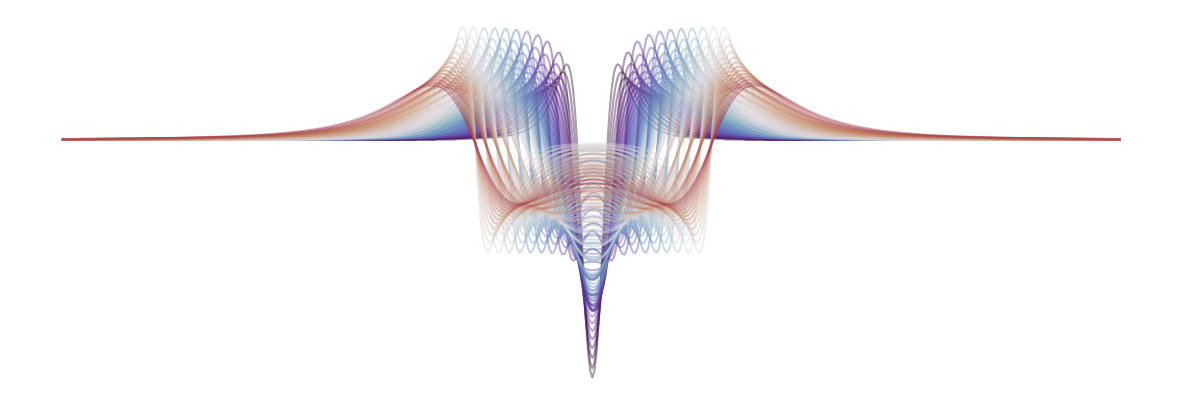
\includegraphics[width=1\linewidth]{images/perfection.png}
    \caption{Dictionnaire local normalisé $\mathbf{D}$ de motifs paramétriques théoriques fournit par RTE d'après l'interpétation de la vérité terrain selon le modèle (\ref{eq:flux}). Les motifs sont centrés et ajustés à la longueur de l'atome le plus long de longueur $L = 492$}
    \label{fig:dictionary}
\end{figure}

\subsection{Modélisation mathématique}

Nous observons un signal $\mathbf{y} \in \mathbb{R}^T$, composé de $T$ échantillons, modélisé comme une composition de plusieurs atomes convolués avec leurs codes d'activation épars respectifs. L'expression pour $\mathbf{y}$ peut être détaillée comme suit :

\begin{equation}
    \mathbf{y} = \sum_{j=0}^{p-1} \mathbf{d}_j * \mathbf{z}_j^\star + \sigma \varepsilon
\end{equation}

où $\{\mathbf{d}_j\}_{j \in \llbracket 0, p-1 \rrbracket}$ représente $p$ atomes de norme unitaire de longueur $L$, chacun convolué avec un signal d'activation parcimonieux correspondant à $\mathbf{z}_j^\star \in \mathbb{R}^{\widetilde{T}}$, et $\sigma \varepsilon$ prend en compte le bruit dans le système. 
Le paramètre $\widetilde{T} = T-L+1$ désigne le nombre de décalages valides pour un atome à l'intérieur du signal, assurant une couverture complète. Pour analyser le signal à travers ces convolutions, nous utilisons une matrice de mesure $\boldsymbol{\Phi} \in \mathbb{R}^{T \times (\widetilde{T}p)}$, construite en concaténant tous les décalages des atomes $\mathbf{d}_j$ sur toute la longueur du signal. 
Cette configuration permet au signal observé $\mathbf{y}$ d'être représenté comme $\boldsymbol{\Phi} \mathbf{Z}^\star$, où $\mathbf{Z}^\star \in \mathbb{R}^{\widetilde{T} p}$ agrège les activations éparses $\mathbf{z}_j^\star$.
La tâche principale est d'estimer précisément ces vecteurs d'activation parcimonieux $\mathbf{Z}^\star$ à partir des observations bruitées de $\mathbf{y}$. Ce défi est intrinsèquement un problème de déconvolution, visant à démêler les effets superposés des activations d'atomes pour récupérer la vraie structure sous-jacente des signaux.


\subsection{Codage convolutionnel parcimonieux}

Les méthodes utilisant la norme $\ell_1$ en codage convolutionnel parcimonieux, convolutional sparse coding en anglais que l'on désignera par la suite par CSC, sont couramment adoptées en raison de leur nature convexe, facilitant le processus d'optimisation dans la décomposition des signaux.
Bien que cette approche induise une parcimonie en minimisant la somme des valeurs absolues des coefficients, elle conduit fréquemment à un nombre excessif d'activations.
La continuité de la norme $\ell_1$, malgré la simplification des calculs, peut compromettre la parcimonie de la solution, en particulier dans des environnements de signaux complexes où une déconvolution précise est essentielle. 

au contraire, les algorithmes gloutons qui exploitent la norme $\ell_0$, tels que Matching Pursuit (MP) et Orthogonal Matching Pursuit (OMP), visent une parcimonie plus stricte en comptabilisant les coefficients non nuls. 
Cette méthode favorise intrinsèquement une représentation plus éparse, cruciale pour la reconstruction de signaux de haute fidélité.
Toutefois, ces techniques basées sur la norme $\ell_0$ se révèlent souvent insuffisantes en termes de capacités de déconvolution, particulièrement lorsqu'elles sont confrontées à des composants se chevauchant dans les signaux. 
En effet, il n'est pas rare que la sélection d'un seul indice incorrect durant le processus de recherche engendre des artefacts dans le résidue et mène à un résultat totalement inexact de l'OMP. 

Le défi persistant en CSC est d'atteindre une déconvolution véritablement parcimonieuse.
Les méthodes actuelles généralisent soit trop avec la norme $\ell_1$, soit déconvoluent de manière inadéquate les signaux se chevauchant avec des algorithmes basés sur la norme $\ell_0$. 
Pour répondre à cela, nous avons adopté une approche combinatoire introduite dans \cite{multipath_matching_pursuit} dénommée le Multipath Matching Pursuit ou MMP, une généralisation de l'Orthogonal Matching Pursuit qui explore des combinaisons d'atomes de façon arborescente pour affiner le processus de sélection glouton. 
Nous avons adapté pour la première fois la MMP au contexte convolutionnel, une approche novatrice à notre connaissance, visant à renforcer l'application de la parcimonie et à améliorer les performances de déconvolution. 
Cette adaptation cible des tâches complexes de traitement de signaux pour parvenir à une compréhension fines des structures sous-jacentes mêmes si elles comportent plusieurs motifs superposés.

\subsection{Contributions}

Ce stage s'est concentré principalement sur l'implémentation de l'algorithme OMP, la mise en évidence de ses limites dans le contexte de la déconvolution sur des intervalles qui présentent de la superposition d'atomes, et l'exploration de solutions innovantes pour surmonter ces défis.
Nous avons proposé une approche de déconvolution parcimonieuse qui combine les avantages de la norme $\ell_0$ avec les capacités de recherche combinatoire de l'approche \textit{multipath}.
Cette contribution se distingue par les points suivants :
\begin{itemize}
    \item \textbf{Adaptation de la stratégie Multipath :} Nous avons adapté les stratégies multipath au contexte convolutionnel en prenant compte de la cohérence élevée des dictionnaires convolutionnels. Cette adaptation assure des interactions plus robustes entre les éléments du dictionnaire et permet d'optimiser le processus de déconvolution.
    \item \textbf{Redéfinition de l'exploration des chemins :} Nous redéfinissons l'exploration de l'espace atomique au sein des dictionnaires convolutionnels, abordant de manière distinctive la gestion de la cohérence. Cette navigation innovante minimise les interférences des caractéristiques se chevauchant, atteignant des représentations parcimonieuses plus fines.
    \item \textbf{Gestion de la complexité :} Notre approche gère efficacement la complexité computationnelle en rationalisant la sélection des atomes et leur réutilisation durant l'exploration des chemins, nous réduisons significativement les demandes computationnelles sans sacrifier la parcimonie ni la précision de la déconvolution.
\end{itemize}
Ces améliorations stratégiques constituent ainsi une avancée méthodologie significative dans le domaine de la déconvolution parcimonieuse, ouvrant la voie à des applications plus complexes nécessitant une analyse plus fine de la structure des signaux.


\section{Etat de l'art}

\subsection{Contexte de la déconvolution gloutonne}

\subsubsection{Corrélations}
Une approche initiale simple pour identifier un motif au sein d'un signal consiste à déterminer quel motif, i.e. quel atome, est le plus corrélé avec le signal.

La corrélation entre $\mathbf{y}$ et les atomes du dictionnaire $\mathbf{D}$ à travers différents décalages est encapsulée dans la matrice $\Phi$, qui est construite en concaténant les versions décalées de $\mathbf{D}$. Le bloc $t$-ième de $\Phi$, noté $\Phi[t]$, contient des colonnes correspondant aux $p$ atomes décalés de $t$ positions. Ainsi, le dictionnaire global $\Phi$ nous permet de calculer efficacement les corrélations pour tous les décalages simultanément.

Sous forme matricielle, la corrélation peut être exprimée comme :
\begin{equation}
    \mathbf{c}_i = \Phi^T \mathbf{y}
\end{equation}
où $\mathbf{c}_i \in \mathbb{R}^{\widetilde{T}}$ est le vecteur des corrélations pour l'atome $\mathbf{d}_i$ à travers tous les décalages possibles. Cette approche simplifie la tâche d'identification de l'atome le plus corrélé, fournissant une base pour la déconvolution et le codage parcimonieux ultérieurs.

\subsubsection{Matching Pursuit}
Le but de l'algorithme Matching Pursuit est de décomposer itérativement un signal en une combinaison linéaire d'atomes provenant d'un dictionnaire, permettant ainsi d'obtenir une représentation parcimonieuse. Dans le contexte de notre problème, l'algorithme Matching Pursuit est utilisée pour identifier et sélectionner les atomes les plus corrélés avec le signal observé $\mathbf{y}$, un à un. Ce faisant, elle affine progressivement l'approximation du signal en soustrayant la contribution des atomes sélectionnés du signal résidu à chaque étape. Ce processus itératif se poursuit jusqu'à ce qu'un critère spécifié, tel qu'un niveau de parcimonie souhaité ou un seuil d'erreur de reconstruction, soit atteint. Finalement, l'algorithme Matching Pursuit vise à récupérer avec précision les signaux d'activation parcimonieux $\mathbf{z}_j^{\star}$, permettant une déconvolution efficace du signal observé et améliorant la reconstruction globale du signal.

\subsubsection{Orthogonal Matching Pursuit}

L'algorithme Orthogonal Matching Pursuit, que l'on désignera par OMP, est un algorithme glouton utilisé pour aborder le problème de l'approximation parcimonieuse dans le traitement des signaux. L'objectif est d'approximer un signal $\mathbf{y}$ comme une combinaison linéaire d'un petit nombre d'atomes provenant d'un dictionnaire $\mathbf{D}$, représentant efficacement le signal avec une erreur résiduelle minimale. L'algorithme OMP procède comme suit :

\begin{rhoenv}[frametitle=Algorithme OMP]
\\
    \textbf{1. Initialisation :} Commencer avec un ensemble vide d'atomes sélectionnés $\mathbf{S} = \emptyset$, un résidu initial $\mathbf{r}_0 = \mathbf{y}$, et fixer le compteur d'itération à $k=0$.
\\\\
    \textbf{2. Sélection d'atome :} À chaque itération, identifier l'atome du dictionnaire qui a la plus haute corrélation avec le résidu courant. Cet atome, noté $\mathbf{d}_{j^*}$, est sélectionné où 
    \begin{equation}
        j^* = \arg \max_j |\langle \mathbf{d}_j, \mathbf{r}_k \rangle|.
    \end{equation}
    Ajouter l'atome sélectionné $\mathbf{d}_{j^*}$ à l'ensemble $\mathbf{S}$.
\\\\
    \textbf{3. Résolution du Problème des Moindres Carrés :} Mettre à jour les coefficients pour les atomes dans $\mathbf{S}$ en résolvant un problème des moindres carrés pour minimiser le résidu étant donné les atomes actuellement sélectionnés :
    \begin{equation}
        \boldsymbol{\alpha} = \arg \min_{\boldsymbol{\alpha}} \|\mathbf{y} - ( \boldsymbol{\Phi} )_{\mathbf{S}} \boldsymbol{\alpha}\|^2.
    \end{equation}
\\\\
    \textbf{4. Mise à jour du résidu :} Mettre à jour le résidu pour l'itération suivante :
    \begin{equation}
        \mathbf{r}_{k+1} = \mathbf{y} - ( \boldsymbol{\Phi} )_{\mathbf{S}} \boldsymbol{\alpha},
    \end{equation}
    où $( \boldsymbol{\Phi} )_{\mathbf{S}}$ est la matrice composée des atomes sélectionnés dans $\mathbf{S}$.
\\\\
    \textbf{5. Vérification de la Convergence :} Vérifier si la norme du résidu est en dessous d'un seuil prédéfini ou si le nombre maximal d'itérations a été atteint. Si ce n'est pas le cas, incrémenter $k$ et répéter à partir de l'étape 2.
\end{rhoenv}


L'algorithme OMP est efficace pour trouver une représentation parcimonieuse du signal, exploitant les corrélations entre le signal observé $\mathbf{y}$ et les atomes du dictionnaire. Ce processus de raffinement itératif assure que les atomes sélectionnés contribuent significativement à la reconstruction du signal, minimisant ainsi l'erreur résiduelle et améliorant la précision de la déconvolution.

\subsection{Complexité de l'OMP dans le contexte convolutionnel}

La complexité de l'algorithme de l'OMP est un aspect critique à considérer pour les problèmes à grande échelle. Les étapes principales impliquent le calcul de la corrélation, la sélection d'atome, l'estimation des moindres carrés et la mise à jour du résidu. Examinons chaque étape en détail, en considérant $k$ comme l'étape courante de l'OMP, c'est-à-dire le nombre d'éléments non nuls dans le vecteur d'activation.

\paragraph{Calcul de la Corrélation}
À chaque itération, l'algorithme calcule la corrélation entre le résidu $\mathbf{r}_k$ et tous les atomes du dictionnaire $\mathbf{D}$ en utilisant une convolution basée sur la FFT. Cela implique :
\begin{equation}
    \mathbf{c}_i = \Phi^T \mathbf{r}_k,
\end{equation}
où $\Phi \in \mathbb{R}^{T \times (\widetilde{T}p)}$. En utilisant la FFT, la complexité de cette opération est réduite à $\mathcal{O}(T \log T \cdot p)$.

\paragraph{Sélection d'Atome}
Sélectionner l'atome avec la plus haute corrélation nécessite de chercher à travers les corrélations calculées. Cette étape a une complexité de $\mathcal{O}(\widetilde{T}p)$.

\paragraph{Problème des Moindres Carrés}
L'étape la plus coûteuse en calcul est la résolution du problème des moindres carrés pour mettre à jour les coefficients pour les atomes sélectionnés. À l'itération $k$, nous résolvons :
\begin{equation}
    \boldsymbol{\alpha} = \arg \min_{\boldson{\alpha}} \|\mathbf{y} - (\boldsymbol{\Phi})_{\mathbf{S}} \boldsymbol{\alpha}\|^2,
\end{equation}
où $(\boldsymbol{\Phi})_{\mathbf{S}}$ est la matrice composée des $k$ atomes sélectionnés. Cela nécessite le calcul de :
\begin{itemize}
    \item Former la matrice de Gram $(\boldsymbol{\Phi})_{\mathbf{S}}^T (\boldsymbol{\Phi})_{\mathbf{S}}$ avec une complexité $\mathcal{O}(Tk^2)$.
    \item Calculer l'inverse ou résoudre le système linéaire, qui a typiquement une complexité $\mathcal{O}(k^3)$.
    \item Multiplier l'inverse par les vecteurs appropriés pour obtenir les coefficients, avec une complexité $\mathcal{O}(Tk)$.
\end{itemize}
Ainsi, la complexité totale pour l'étape des moindres carrés à l'itération $k$ est $\mathcal{O}(Tk^2 + k^3)$.

\paragraph{Mise à Jour du Résiduel}
Mettre à jour le résiduel implique de calculer :
\begin{equation}
    \mathbf{r}_{k+1} = \mathbf{y} - (\boldsymbol{\Phi})_{\mathbf{S}} \boldsymbol{\alpha},
\end{equation}
qui a une complexité de $\mathcal{O}(Tk)$.

\paragraph{Complexité Globale}
En supposant que $k \ll T$ et notant que l'algorithme fonctionne typiquement pour $K$ itérations (où $K$ est le niveau de parcimonie du signal que nous cherchons à récupérer), nous pouvons additionner les complexités des étapes individuelles sur toutes les itérations. Le terme dominant est le calcul des moindres carrés. Ainsi, la complexité globale de l'OMP peut être approximée comme :
\begin{equation}
    \mathcal{O}(K \cdot (T \log T \cdot p + Tk^2 + k^3)) = \mathcal{O}(KT \log T \cdot p + TK^3 + K^4).
\end{equation}

Étant donné que $k \ll T$, la complexité peut être largement résumée comme $\mathcal{O}(KT \log T \cdot p + TK^3)$, mettant en évidence la dépendance à la longueur du signal $T$, au nombre d'atomes $p$, et au niveau de parcimonie $K$.

Dans le cas convolutionnel, il est typique que $T \gg K$, i.e. que $\log T \gg K$. De plus, nous avons généralement $p \gg K$ car nous recherchons quelques atomes paramétriques parmi un grand nombre de paires de paramètres $p$. Par conséquent, le terme $KT \log T \cdot p$ est grand devant le terme $TK^3$, nous permettant de simplifier davantage la complexité globale.

Ainsi, la complexité globale simplifiée de l'algorithme OMP dans le contexte convolutionnel peut être exprimée ainsi :
\begin{equation}
    \textit{OMP Convolutionnel} \equiv O(KT \log T \cdot p).
\end{equation}


\subsection{Les limites de l'OMP}

L'OMP rencontre des défis significatifs dans la déconvolution, notamment lorsqu'elle doit gérer plusieurs atomes superposés. 
La nature gloutonne de l'OMP consiste à privilégier l'atome le plus corrélé à chaque étape. Or cela échoue souvent à séparer avec précision les motifs superposés.  
En conséquence de quoi la performance de l'OMP est fortement détériorée, menant à une reconstruction du signal sous-optimale et donc à une mauvaise déconvolution.

\begin{figure}[H]
    \centering
    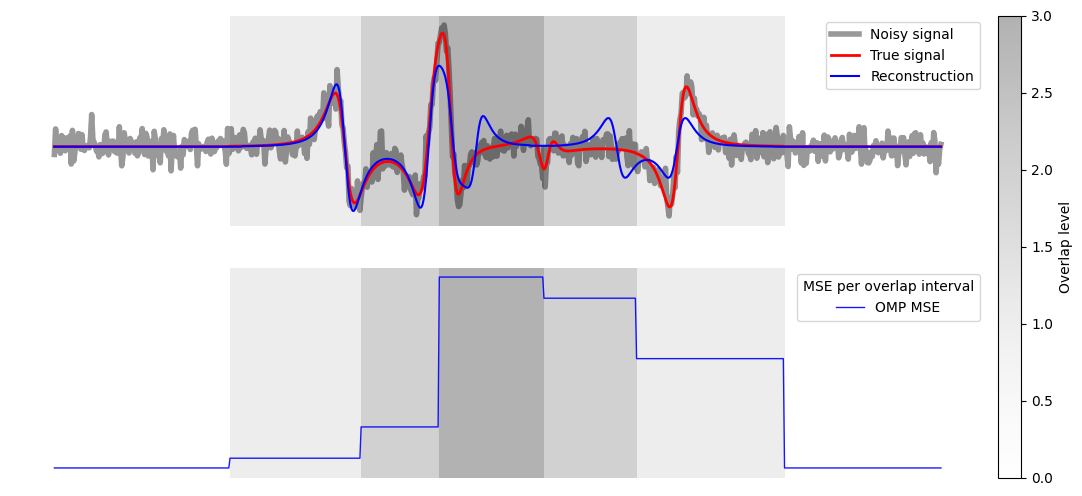
\includegraphics[width=1\linewidth]{images/omp_overlap_mse.png}
    \caption{Mise en évidence de l'augmentation significative de l'erreur de déconvolution dans les intervalles avec des atomes superposés pour l'OMP.}
    \label{fig:omp_overlap}
\end{figure}

\subsection{Intérêt d'une approche combinatoire arborescente}

Une question cruciale se pose : comment réaliser une déconvolution efficace en utilisant une approche gloutonne telle que l'OMP ? 
Au lieu de se servir de l'OMP comme simple point de départ, nous pouvons contourner sa propension à la gloutonnerie en explorant des voies alternatives. 
En sélectionnant les atomes qui sont les deuxième ou troisième plus corrélés, nous pouvons naviguer à travers plusieurs branches de solutions potentielles. 
Cette exploration combinatoire peut révéler une branche offrant une reconstruction nettement améliorée. 
Cela nous conduit au Multipath Matching Pursuit \cite{multipath_matching_pursuit}. Avec une augmentation constante de la complexité, nous pouvons significativement renforcer la capacité de déconvolution. 
En explorant systématiquement ces chemins alternatifs, nous pouvons parvenir à une reconstruction du signal beaucoup plus précise. 
Cela prépare le terrain pour l'algorithme MMP, qui sera détaillé dans la section suivante.

\newpage

\section{La Méthode \textit{Multipath}}

\subsection{Concept du Multipath Matching Pursuit}

Le concept fondamental du Multipath Matching Pursuit, que l'on désignera par la suite par MMP, implique l'exécution de multiples OMPs, chacun explorant des chemins différents en sélectionnant divers atomes corrélés à chaque itération. Au lieu de se limiter à l'atome le plus corrélé, la MMP envisage plusieurs candidats prometteurs, se ramifiant ainsi en plusieurs solutions possibles. Cette approche permet à l'algorithme de maintenir plusieurs chemins de reconstruction, augmentant la probabilité de trouver une déconvolution plus précise et robuste du signal.

\begin{rhoenv}[frametitle=La stratégie \textit{depth-first}]
    L'algorithme de Multipath Matching Pursuit est disponible en deux variantes :
    \begin{itemize}
        \item \textbf{MMP \textit{breadth-first} (MMP-BF)} : MMP-BF explore plusieurs chemins candidats en parallèle, ce qui, bien que complet, entraîne une surcharge computationnelle importante, surtout à mesure que la dimensionnalité des atomes augmentent.
        \item \textbf{MMP \textit{depth-first}  (MMP-DF)} : En revanche, MMP-DF adopte une stratégie de recherche séquentielle, ce qui simplifie grandement la gestion de la charge computationnelle en limitant le nombre de chemins explorés.
    \end{itemize}
\end{rhoenv}


L'approche MMP-DF est particulièrement avantageuse dans les contextes convolutionnels où les atomes présentent des degrés élevés de corrélation entre eux. En employant une recherche en profondeur d'abord, MMP-DF se concentre sur l'exploration des chemins les plus prometteurs dès le début du processus de recherche, évitant ainsi les écueils des calculs redondants inhérents à la stratégie MMP-BF.

\subsection{Premiers pas}
La première approche de la MMP introduit le concept de \emph{branche}, qui est similaire à une exécution complète de l'OMP. 
Chaque chemin est une exécution de l'OMP qui, à certaines étapes, sélectionne les deuxième ou troisième atomes les plus corrélés au lieu de toujours prendre l'\textit{argmax}. 
Cette stratégie de branchement permet à la MMP d'explorer un espace combinatoire de solutions potentielles. 
Pour formaliser cela, soit $L$ le nombre de chemins explorés par nœud. 
Pour la branche $\ell$-ième à l'étape $k$, nous désignons le résidu par $\mathbf{r}_{\ell}^k$. À chaque nœud de l'arbre de recherche, MMP-DF sélectionne $L$ atomes différents à explorer, créant ainsi $L$ nouvelles branches. Ce processus est répété de manière itérative, maintenant et mettant à jour les résidus $\mathbf{r}_i^k$ pour chaque branche. Chaque résidu est associé à un atome voir table \ref{table:mmp-df}.
\renewcommand{\arraystretch}{1.6} % Ajuster l'espacement des lignes

%\begin{table}[h]

\subsection{Contexte convolutionnel}
Dans les scénarios convolutionnels, le défi critique réside dans la bonne ramification entre les nœuds de recherche de l'arbre en raison de la forte cohérence de la matrice de mesure $\boldsymbol{\Phi}$. Les corrélations entre les atomes émanent de variations paramétriques minimes dans la forme des atomes et leurs décalages positionnels dans le signal, rendant problématique la distinction efficace entre atomes similaires. En conséquence, la recherche du deuxième ou du troisième atome le plus corrélé aboutit souvent à la sélection d'atomes presque identiques au premier, perpétuant les mêmes biais et artefacts dans les résidus subséquents. Pour contourner ce problème, une nouvelle contrainte est nécessaire dans les cas convolutionnels, que nous nommons la \textit{contrainte de dissimilarité}. Considérons l'exploration de la branche $\ell$-ème à l'étape $k$ telle que $\ell < N_{\text{max}}$ et $k < K$. Le problème est théoriquement exprimé comme la recherche des $L$ atomes les plus corrélés avec le résidu local $\mathbf{r}_i^k$ qui sont mutuellement décorrélés selon un seuil de décorrélation $\delta$ :
\begin{align}
    \mathcal{J}_{\ell}^k &= \underset{\mathcal{J} \in \llbracket 1, \Omega \rrbracket^L}{\operatorname{argmax}} \Big\| \big( \boldsymbol{\Phi}^T  \mathbf{r}_{\ell}^k \big)_\mathcal{J} \Big\|_2^2 \notag \\
    \text{s.t.} &\quad \forall (i, j) \in \mathcal{J}, i \neq j \Rightarrow \big | \big \langle \boldsymbol{\Phi}[i],  \boldsymbol{\Phi}[j] \big \rangle \big | < \delta
    \label{eq:dissimilarity}
\end{align}

Le paramètre \(\delta\), définissant la contrainte de dissimilarité, doit être ajusté avec soin selon chaque cas spécifique, dépendant largement des caractéristiques de cohérence de la matrice de mesure \(\boldsymbol{\Phi}\). Pour fixer le paramètre $\delta$ une approche empirique est adoptée : on constate que pour $\delta = 0.4$ on maximise le nombre de vrais positifs sur un dataset synthétique. le choix n'est pas évident car pour un seuil $\delta \in [0.4, 0.7]$ les performances sont comparables. Par la suite on considèrera donc que $\delta = 0.4$.

\subsection{Raffinement de la complexité}
Le raffinement computationnel de cette approche repose sur le nombre de nœuds calculés à chaque niveau de l'arbre et l'étendue de la réutilisation des calculs précédents. Un nœud représente une itération dans une branche, chacune associée à un résidu et un indice d'atome.

\begin{itemize}
    \item Pour les premières \(L\) branches, chaque branche nécessite le calcul de \(K\) nœuds, aucune computation antérieure ne pouvant être réutilisée.
    
    \item Pour les \(L(L-1)\) branches suivantes, chaque branche calcule seulement \(K-1\) nœuds car le résultat du nœud racine des calculs précédents est réutilisé.
    \item En continuant selon ce modèle, pour les branches suivantes \(L(L-1)(L-2)\), seulement \(K-2\) nœuds nécessitent un calcul, en tirant parti de deux niveaux de résultats précédemment calculés.
    \item Pour les branches finales, un seul nouveau nœud est calculé par branche, utilisant le maximum de nœuds calculés précédemment jusqu'à \(K-1\).
\end{itemize}
En supposant que le coût computationnel de l'évaluation d'un seul nœud est $\mathcal{O}( T \log T \cdot p)$, où $p$ représente le nombre d'atomes locaux et $T$ la longueur du signal, la complexité totale $C$ peut s'exprimer ainsi $ C = L \cdot K \cdot \mathcal{O}(T \log T \cdot p) + L(L-1) \cdot (K-1) \cdot \mathcal{O}(T \log T \cdot p) + \ldots $.

En simulation on retrouve le fait que le nombre de noeuds calculés connait une décroissance exponentielle en fonction du numéro de la branche explorée comme le montre la figure \ref{fig:computation_deconv}.
\begin{figure}[H]
    \centering
    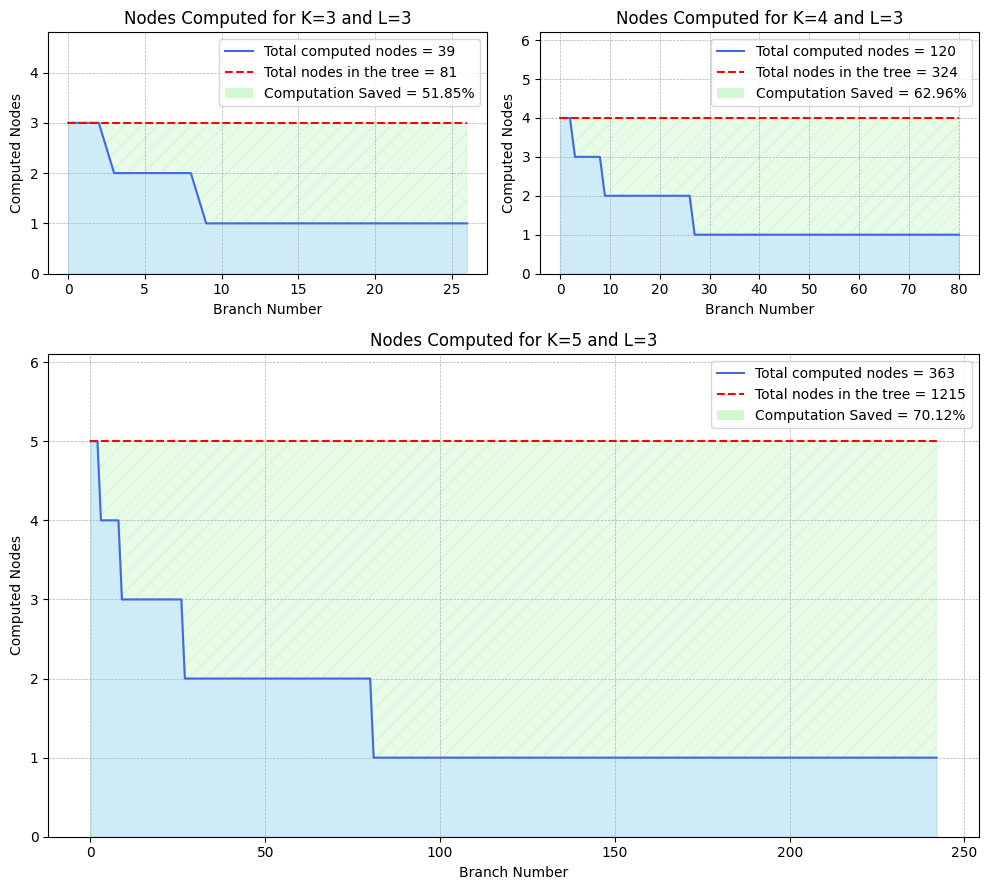
\includegraphics[width=0.8\linewidth]{images/mmpdf_computation.png}
    \caption{Nombre de noeuds calculé en fonction du numéro de la branche courante pour $L=3$ et $K \in \{3, 4, 5 \}$.}
    \label{fig:computation_deconv}
\end{figure}

\newpage

\section{Expérience}

\subsection{Dictionnaire}

Le dictionnaire utilisé est élaboré à partir des formulations de Zatsepin et Schcherbinin ainsi que des mesures de référence effectuées par RTE. Il illustre les variations du paramètre $y$ en abscisse et du paramètre $b$ en ordonnée, tandis que le paramètre $\sigma$ est ajusté pour normaliser les amplitudes des atomes.


\begin{figure}[H]
    \centering
    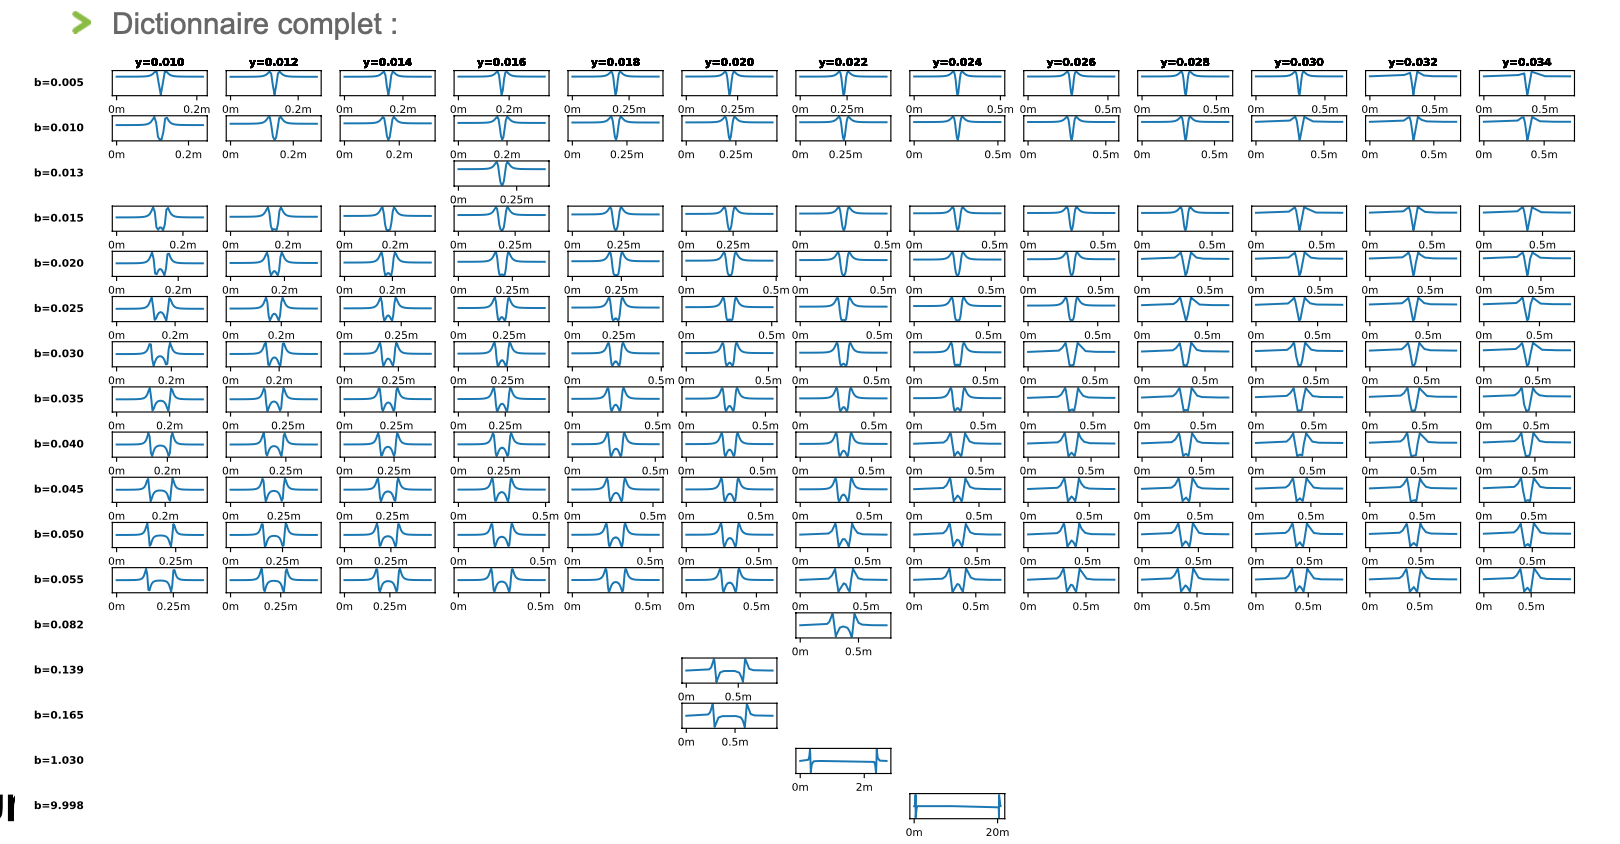
\includegraphics[width=\linewidth]{images/dictionnaire_rte.png}
    \caption{Dictionnaire de formes d'ondes paramétriques fournit par RTE : $b_{min} = 0.005$, $b_{max} = 0.06$, $b_{step} = 0.005$, $y_{min} = 0.010$, $y_{max} = 0.036$, $y_{step} = 0.002$.}
    \label{fig:dict_rte}
\end{figure}

Les atomes, tendant vers zéro de part et d'autre d'une zone centrale d'activation, sont caractérisés par une longueur $L$, définie comme l'étendue hors de laquelle leur amplitude demeure inférieure à un seuil arbitraire $\zeta=0.001$. 
Compte tenu de leurs formes variées, les atomes présentent des longueurs différentes; ils sont ainsi alignés sur la longueur de l'atome le plus long par l'ajout de zéros aux extrémités. 
Ce processus aboutit à un dictionnaire composé de 143 atomes, chacun d'une longueur de 492 unités, et les atomes sont normalisés pour en faciliter la comparaison en ajustant le paramètre $\sigma$ pour chaque atome.


\subsection{Données synthétiques}

La génération de données synthétiques se fait par sélection aléatoire d'atomes dans le dictionnaire susmentionné. 
Nous constituons un signal dont la longueur est 1,5 fois celle des atomes afin de permettre des décalages variés entre ceux-ci, évaluant ainsi notre algorithme dans des configurations présentant des superpositions diverses. 
Pour instaurer des conditions réalistes, il est stipulé que les atomes ne soient pas positionnés à moins de 10 pas les uns des autres et qu'ils affichent une corrélation inférieure à 0.75 en valeur absolue.

Cette contrainte imite les conditions physiques du problème; si des atomes identiques se superposent parfaitement, il devient impossible de les distinguer, obligeant ainsi à reconsidérer la définition de nouveaux paramètres $(b, y, \sigma)$. Le signal généré comprend aléatoirement $K$ atomes parmi les 143 disponibles, disposés sur 246 décalages possibles, permettant à chaque atome d'être intégré au signal. 
Un bruit gaussien est ensuite ajouté, la variance étant ajustée pour fixer un rapport signal sur bruit (SNR) déterminé par l'équation suivante :
$$
\mathrm{SNR}=10 \log _{10}\left(\frac{\|\mathbf{y}\|_2^2}{\|\mathbf{y}-\hat{\mathbf{x}}\|_2^2}\right)
$$

Cette procédure est réitérée pour obtenir toutes les combinaisons possibles avec $K \in\{2,3,4,5\}$ et $S N R \in\{0 \mathrm{~dB}, 5 \mathrm{~dB}, 10 \mathrm{~dB}, 15 \mathrm{~dB}\}$. 
En résultent 200 signaux synthétiques pour chaque couple $(K, S N R)$, totalisant ainsi 3200 signaux synthétiques sur lesquels notre algorithme est évalué.


\subsection{Métriques}

Dans le contexte du codage convolutionnel parcimonieux, l'erreur quadratique moyenne (MSE) constitue une métrique initiale permettant d'évaluer la performance de l'algorithme. 
Si une MSE élevée indique clairement une défaillance de l'algorithme, une MSE faible, en revanche, ne garantit pas nécessairement une déconvolution réussie. 
En effet, différentes combinaisons d'atomes peuvent conduire à une reconstruction similaire du signal, masquant ainsi les véritables dynamiques sousjacentes.

Afin d'appréhender plus précisément la qualité de la déconvolution, il est impératif d'introduire une seconde métrique qui évalue la conformité entre les atomes sélectionnés et les atomes réels présents dans le signal. 
Cette évaluation est une mesure de classification au sein d'un espace comportant autant de classes qu'il existe d'atomes distincts dans le dictionnaire global, c'est-à-dire de colonnes dans la matrice de mesure $\mathbf{\Phi}$.

Les variations minimes en termes de position et de forme des atomes peuvent compliquer la distinction entre des atomes similaires, dont les tracés sont parfois presque indiscernables. 
C'est dans ce contexte qu'une métrique de classification devient cruciale pour identifier correctement un vrai positif parmi les différentes classes. 
Pour ce faire, une définition arbitraire de la similarité entre les atomes est adoptée : deux atomes sont considérés comme similaires si leur écart de position est inférieur à cinq pas en valeur absolue et que leur corrélation dépasse un seuil défini, $\delta=0.95$.

La figure ci-dessous découle du résultat de l'OMP et de la MMP sur un signal bruité comportant des motifs superposés. En appliquant un algorithme d'appariemment hongrois en position et en corrélation on peut associer un atome réel avec son approximation par l'algorithme. On constate ici que malgré le fait que l'OMP trouve un atome à une position à moins de cinq pas en valeur absolue de l'atome réel sa corrélation avec ce-derneir ne permet pas de considérer l'atome retrouvé comme un vrai positif. 
Dans cet exemple l'algorithme MMP trouve pour cet atome une solution considéré comme un vrai positif d'après le critère précédent.

\begin{figure}[H]
    \centering
    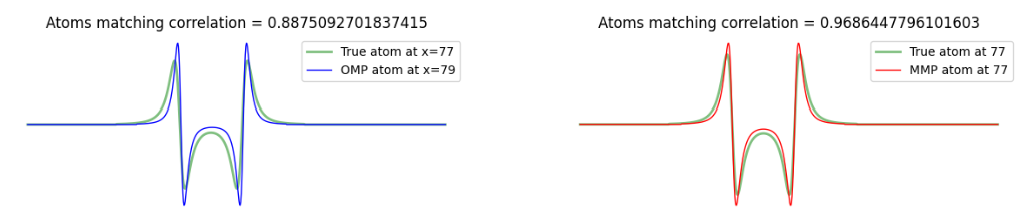
\includegraphics[width=\linewidth]{images/atom_matching.png}
    \caption{A gauche un faux positif et à droite un vrai positif.}
    \label{fig:atom_matching}
\end{figure}

\subsection{Données réelles}

Les données rélles comprennent quinze câbles, dont les longueurs varient de 4,5 m à 22 m, totalisant 248 mètres. Cette diversité offre un panel représentatif des défis rencontrés dans la maintenance des infrastructures énergétiques.

Les données réelles n'offrent pas d'information de référence concernant la position exacte ou les caractéristiques spécifiques des défauts. Ainsi, pour valider la précision de notre algorithme, chaque câble a été mesuré à trois reprises, garantissant que la méthode de mesure est répétable et fiable. Cette répétition nous permet de vérifier la consistance de l'algorithme à détecter les mêmes défauts prototypiques à travers différentes sessions de mesure, illustrant ainsi sa robustesse face au bruit et à la variabilité des conditions de mesure.

L'analyse des résultats sur les données réelles dépasse le cadre de ce stage, il est prévu que l'algorithme développé soit utilisé pour des évaluations plus poussées sur les données réelles. L'objectif à long terme est de confirmer la fiabilité et l'efficacité de cette approche dans des conditions opérationnelles, en assurant une maintenance prédictive précise et économiquement viable des réseaux de transport d'électricité. Cette démarche s'inscrit dans une perspective de durabilité et de renforcement de la sécurité des infrastructures énergétiques, alignée avec les impératifs contemporains de gestion et de préservation des ressources énergétiques.

\newpage
\section{Résultats}

\begin{rhoenv}[frametitle=Considérations pratiques]
    L'exécution de l'algorithme MMP est caractérisée par trois paramètres :
    \begin{itemize}
        \item $K = \texttt{sparsity}$ : le nombres d'atomes que l'algorithme cherche à trouver dans le signal. C'est-à-dire le nombres de noeuds d'une branche de l'arbre de recherche.
        \item $L = \texttt{connections}$ : le nombre d'options que considère l'algorithme pour un résidu donné en comptant l'atome le plus corrélé. C'est-à-dire le nombre de branchements en chaque noeud de l'arbre de recherche.
        \item $N = \texttt{branches}$ : le nombre de branches complètes qu'explore l'algorithme MMP selon la stratégie \textit{depth-first}. C'est-à-dire le nombre d'OMP équivalente que calcule la MMP. Par soucis de clarté on désigne par MMP-$N$ l'algorihme MMP à $N$ branches.
    \end{itemize}
    On remarque que l'algorithme MMP-1 est strictement équivalent à l'OMP. On note de plus que pour $L=3$, MMP-3 consiste en l'exploration des branches issuent de toutes les alternatives offerte par la première couche de l'arbre, MMP-9 explore toutes les alternatives offertes par les deux premières couches, MMP-27 les trois premières couches, et MMP-81 les 4 premières couches.
\end{rhoenv}

\subsection{Erreur de reconstruction} 

En premier lieu on constate que l'exploration de branche issues de corrélations sous-optimales permet bien une meilleure reconstruction finale en bout de branche comme le montre le résultat de la MMP-3 sur le signal de la figure \ref{fig:omp_overlap}.

\begin{figure}[H]
    \centering
    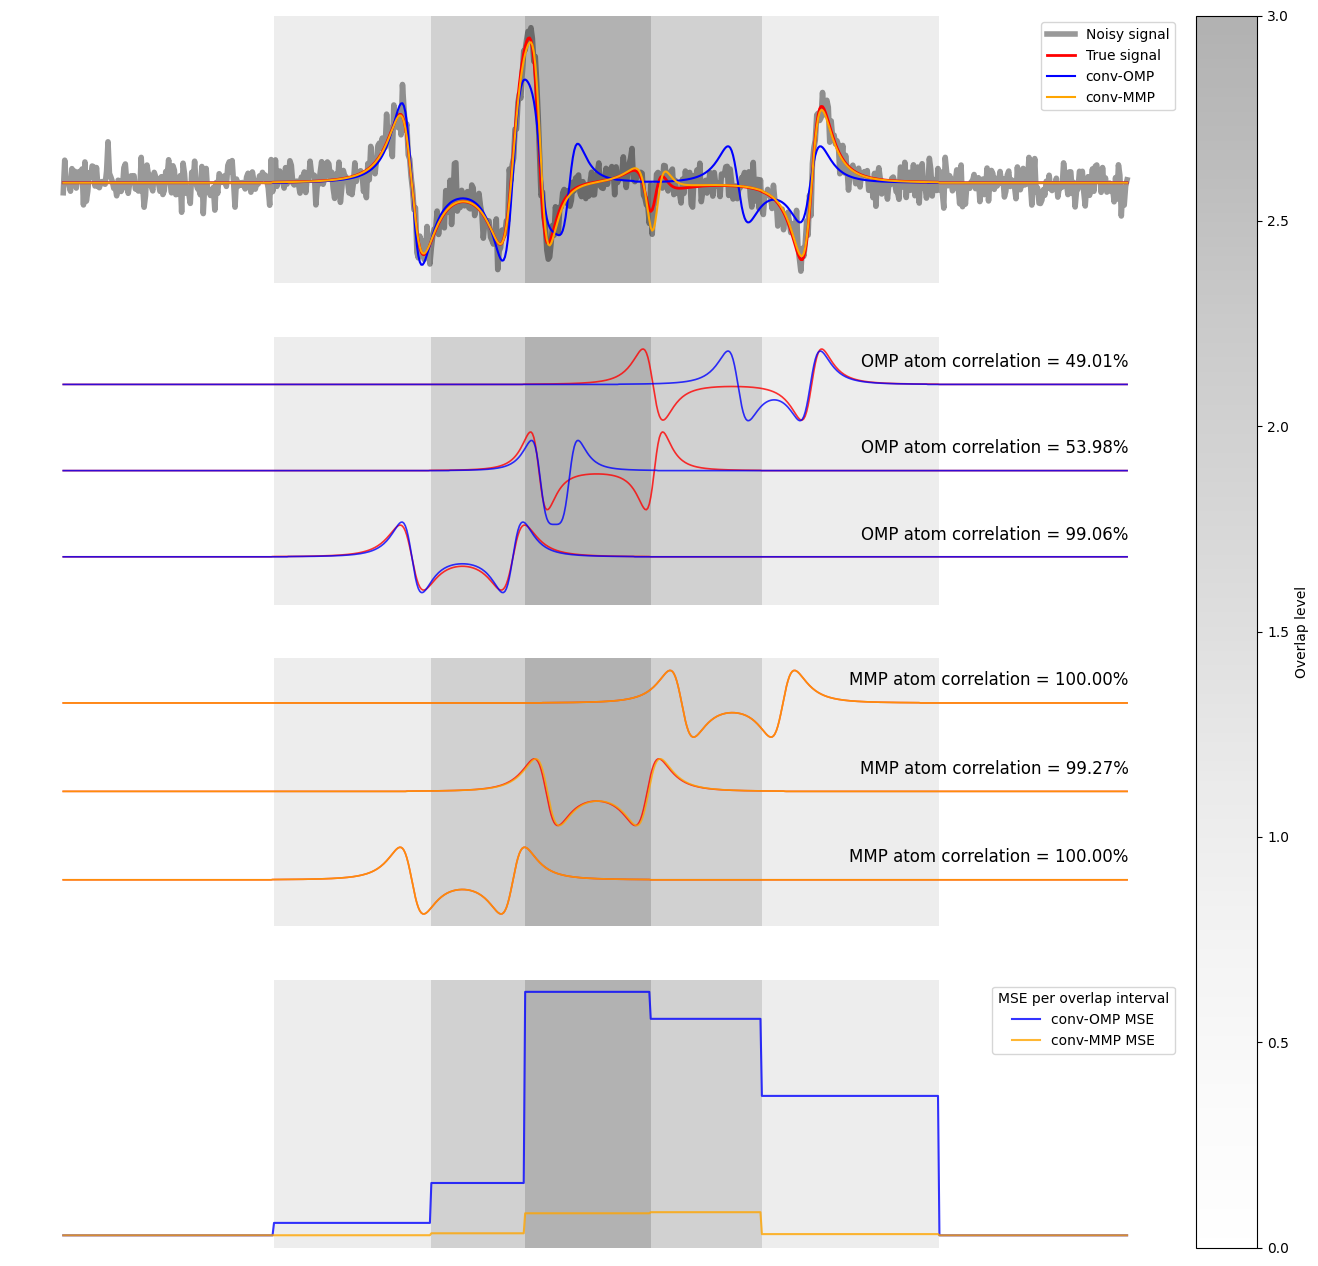
\includegraphics[width=1\linewidth]{images/mmp_overlap_decomposition_v2.png}
    \caption{Comparaison de l'amélioration de l'erreur de déconvolution dans les intervalles avec des atomes superposés.}
    \label{fig:comp_deconv}
\end{figure}

Pour mesurer la performance de la MMP par rapport à l'OMP en ce qui concerne l'erreur de reconstruction sur les intervalles présentant des atomes superposés on trace l'erreur de reconstruction locale pour des intervalles iso-densité d'atomes, c'est-à-dire qu'on construit l'erreur quadratique moyennée sur des intervalles du signal où se superposent une quantité d'atomes donnée.
On construit ces mesures à partir des signaux comportant exactement 5 atomes et une SNR de 10 dB.
On compare l'OMP, les MMP-3, MMP-9, MMP-27 et MMP-81, c'est-à-dire les MMP avec respectivement $3^1$, $3^2$, $3^3$ et $3^4$ branches explorées.
Autrement dit on utilise des MMP qui explore toute les branches possibles jusqu'à une profondeur donnée correspondant $\log_L(N) = \log_3(N)$ avec $N$ le nombre de branches explorées.

\begin{figure}[H]
    \centering
    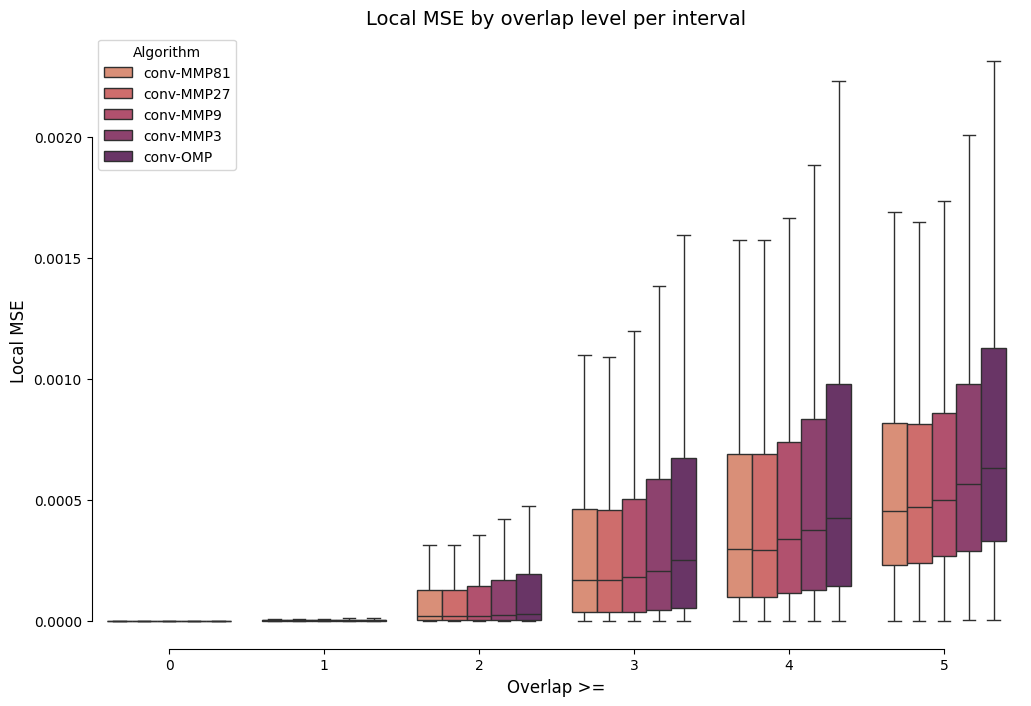
\includegraphics[width=1\linewidth]{images/boxplot_mse.png}
    \caption{Comparaison de l'erreur de reconstruction en fonction de la densité d'atome superposés par intervalle.}
    \label{fig:boxplot_mse}
\end{figure}

La figure ci-dessus met en évidence le fait que l'erreur de reconstruction diminue significativement à mesure qu'on explore plus profondément l'arbre de recherche.

On constate que l'écart se creuse entre la MMP et l'OMP quand il s'agit d'intervalles comportant de plus en plus d'atomes superposés.
On observe de plus une certaine scalabilité de l'algorithme MMP, en effet celui-ci permet en moyenne une meilleure reconstruction du signal à mesure qu'on explore plus de branches dans l'arbre de recherche.
Il est donc possible de contourner le caractère glouton de l'algorithme MMP on sélectionnant de façon locale un atome sous-optimal.
On obsere de plus une forme de convergence puisque les erreurs de reconstruction entre la MMP-27 et la MMP-81 sont significativement les mêmes alors que la MMP-81 explore toute une couche supplémentaire dans l'arbre de recherche.
Cette convergence s'explique par le fait que les erreurs accumulées dans les étapes précédentes ne permettent plus de compenser le gain potentiel à la reconstruction que permet la sélection locale d'un atome sous-optimal.


\subsection{Erreur de déconvolution} % Performance recherché : position & corrélation

Comme expliqué précédemment l'erreur de reconstruction est symptomatique d'une déconvolution efficace mais il n'en est pas le garant.
Pour mesurer de façon clair l'amélioration que permet l'algorithme MMP en matière de déconvolution il est nécessaire de comparer les atomes qui sous-tendent la reconstruction par la MMP.
Nous pouvons ensuite mesurer le nombre de vrais-positifs à l'aide de critère de discernement impliquant l'erreur de position en valeur absolue et la corrélation.
Dans le contexte convolutionnel la mesure de la classification est ambigue car chaque atome à une positon donnée peut-être considéré comme une classe. En conséquence de quoi dès qu'il y a un peu de bruit ou de la superposition la précision des algorithmes OMP et des algorithme MMP s'effondrent puisqu'il est très rare que l'algorithme arrive à tomber exactement sur la bonne position et le bon atome.
Notre critère de discernement permet ainsi de simplifier la classification des atomes tout en s'adaptant aux exigences de la vérité terrain, en effet il n'est en aucun cas question de reconstruire parfaitement le défaut du câble étant donné que les atomes que nous recherchons sont issus de modélisations physiques qui ne représente pas avec exactitude ce que sont les défauts présents dans les câbles.

\newpage

\subsubsection{Critical difference diagram}

Nous souhaitons démontrer que la classification que permet l'algorithme MMP est \textit{significativement} meilleure que la classification permise par l'OMP. Pour ce faire, nous avons recours à un \textit{diagramme de différence critique}, un outil spécialement conçu pour mesurer la performance de classifieurs dans des cas complexes.

\begin{rhoenv}[frametitle=Méthode de construction du diagramme]
    \begin{itemize}
        \item \textbf{Calcul des rangs moyens :} Les performances de chaque classifieur sont évaluées sur plusieurs ensembles de données. Le rang moyen est calculé pour chaque classifieur, en fonction de sa performance relative sur l'ensemble des jeux de données.
        \item \textbf{Application des tests statistiques :} Un test de Friedman est d'abord réalisé pour déterminer si des différences significatives existent entre les classifieurs. Si le test est significatif, un test post-hoc de Nemenyi est ensuite utilisé pour comparer les paires de classifieurs et identifier les différences significatives entre leurs performances.
        \item \textbf{Représentation dans le diagramme :} Les classifieurs dont les performances ne montrent pas de différences significatives sont reliés par une ligne épaisse dans le diagramme, indiquant que leur performance est statistiquement indiscernable.
    \end{itemize}
\end{rhoenv}

Le diagramme de différence critique souligne de façon marquée la supériorité des méthodes basées sur la norme \(\ell_0\) par rapport à la méthode CSC-\(\ell_1\), qui se positionne significativement en retrait en termes de rang moyen. Ce constat illustre l'efficacité remarquable des techniques exploitant la parcimonie stricte dans le traitement de signaux complexes.

Il est également notable que parmi les algorithmes fondés sur la norme \(\ell_0\), même si MMP-3 ne propose que l'exploration de deux branches supplémentaires par rapport à l'OMP, il se distingue nettement tant de l'OMP que de l'OMP se différencie du MP. Cette différence significative met en lumière la puissance de l'approche MMP-3, confirmant son efficacité même avec un nombre limité de branches explorées.

Cette observation renforce le caractère \textit{scalable} de l'algorithme MMP : à mesure que le nombre de branches explorées augmente, on observe une amélioration manifeste de la déconvolution. Ce phénomène est clairement visible dans le diagramme où les performances continuent de s'accroître jusqu'à MMP-27.

Cependant, une forme de convergence est observable entre MMP-27 et MMP-81, connectés par une ligne épaisse, indiquant qu'une augmentation du nombre de branches au-delà de 27 n'entraîne pas nécessairement de gains significatifs en termes de déconvolution. Ce plateau suggère que les bénéfices de l'augmentation du nombre de branches atteignent une limite, au-delà de laquelle les améliorations deviennent marginales.

Ainsi, le diagramme de différence critique offre une visualisation précise et quantifiée de l'impact de la stratégie de parcimonie et du nombre de solutions explorées sur la performance de déconvolution, mettant en exergue l'efficacité et la pertinence des méthodes basées sur la norme \(\ell_0\), la supériorité de la MMP par rapport à l'OMP ainsi que sa grande adaptabilité dans des contextes complexes.

\begin{figure}[H]
    \centering
    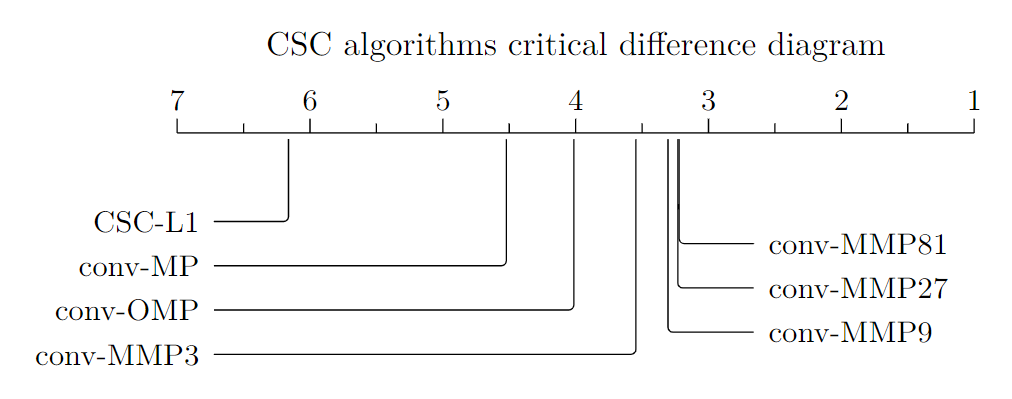
\includegraphics[width=1\linewidth]{images/critical_difference_diagram.png}
    \caption{\textit{Critical difference diagram} illustrant la performance des algorithmes de déconvolution.}
    \label{fig:cdd}
\end{figure}

\subsubsection{Compromis Complexité-Performance}

Dans le contexte du codage convolutionnel parcimonieux, il est essentiel de considérer non seulement l'efficacité des algorithmes en termes de précision de classification mais il est essentiel de considérer leur coût en termes de temps de calcul. 

\paragraph{Analyse de l'erreur quadratique moyenne (MSE)}

Le premier graphique montre l'erreur quadratique moyenne (MSE) en fonction du temps de calcul pour les algorithmes OMP, MMP-3, MMP-9, MMP-27 et MMP-81, avec le temps indiqué en secondes sur l'axe des abscisses et la MSE représentée par des bougies sur l'axe des ordonnées. Chaque bougie illustre la médiane et la variance des performances de chaque algorithme pour un temps de calcul donné.

Bien que la MSE suggère une déconvolution efficace, elle ne garantit pas une performance parfaite. Le graphique montre que le temps de calcul croît presque logarithmiquement à mesure que le nombre de branches explorées triple, passant d'une seule pour l'OMP à 81 pour la MMP-81. Pourtant, les augmentations de temps ne sont pas proportionnelles à l'augmentation des branches; par exemple, MMP-9 requiert moins de 20 secondes pour 9 branches, alors que MMP-27 en explore 27 en moins de 40 secondes, grâce à une réutilisation efficace des nœuds déjà calculés.

On constate également que la précision de la reconstruction s'améliore significativement à mesure que le temps de calcul augmente, ce qui témoigne de l'adaptabilité de l'algorithme MMP à des contextes de déconvolution plus complexes, où des temps de calcul plus longs permettent de parvenir à des solutions plus précises.

\begin{figure}[H]
    \centering
    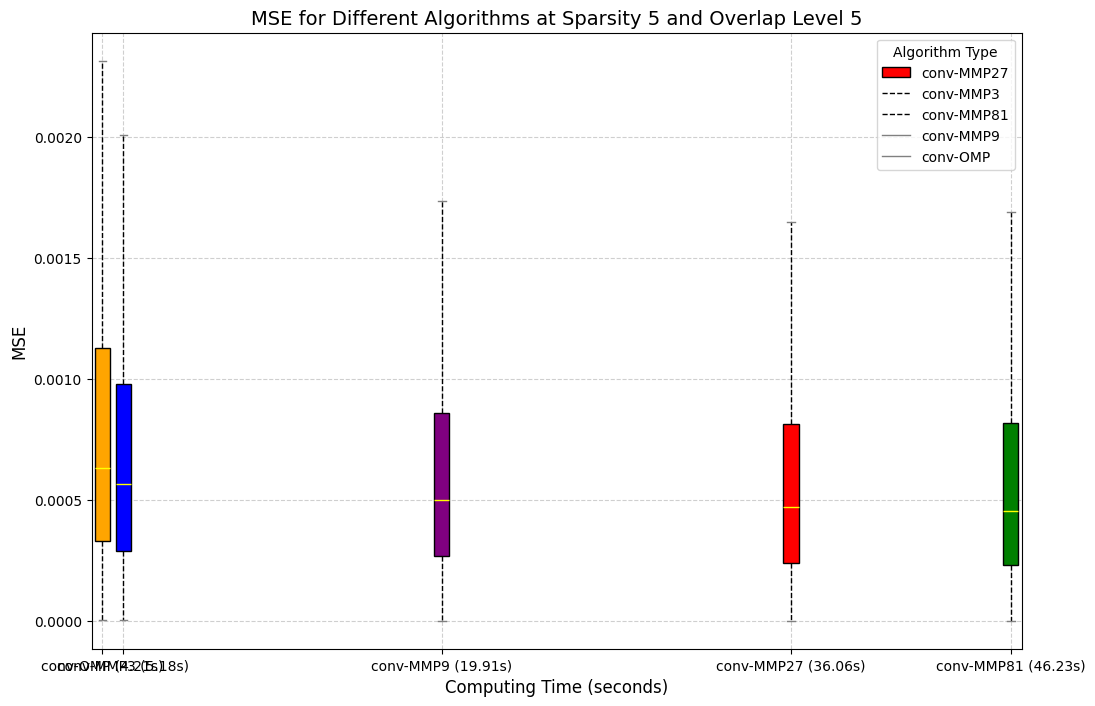
\includegraphics[width=1\linewidth]{images/trade_off_mse.png}
    \caption{Compromis entre l'erreur de reconstruction et le temps de calcul pour les algorithmes de déconvolution.}
    \label{fig:trade_off_mse}
\end{figure}

\newpage

\paragraph{Analyse du score F1}

Le score F1 est une métrique utilisée fréquemment pour évaluer la précision des tests de classification. Il prend en compte à la fois la précision et le rappel pour fournir une mesure harmonique de la performance globale du classificateur. La précision représente la proportion de vrais positifs par rapport au total des cas classés positivement, tandis que le rappel mesure la proportion de vrais positifs par rapport au nombre total de cas réellement positifs dans les données.

\begin{itemize}
    \item \textbf{Précision :} La précision est le rapport entre le nombre de vrais positifs et le nombre de tous les positifs prédits (vrais positifs plus faux positifs).
    \[ \text{Précision} = \frac{TP}{TP + FP} \]
    \item \textbf{Rappel :} Le rappel est le rapport entre le nombre de vrais positifs et le nombre de positifs réels (vrais positifs plus faux négatifs).
    \[ \text{Rappel} = \frac{TP}{TP + FN} \]
    \item \textbf{Score F1 :} Le score F1 est la moyenne harmonique de la précision et du rappel, ce qui permet de tenir compte à la fois de la précision et du taux de récupération des cas positifs.
    \[ F1 = 2 \times \frac{\text{Précision} \times \text{Rappel}}{\text{Précision} + \text{Rappel}} \]
\end{itemize}

Le graphique du score F1 en fonction du temps de calcul met en lumière l'efficacité relative des algorithmes de déconvolution en termes de précision et de rappel, des métriques cruciales pour les tâches de classification. Ce graphique confirme que les améliorations obtenues avec les algorithmes MMP, notamment MMP-27 et MMP-81, augmentent le temps de calcul mais offrent des gains significatifs en termes de performance de classification.

Notamment, on observe que la précision de l'OMP se situe autour de 20\%, tandis que pour les variantes MMP, elle atteint 30\% selon le même critère de discernement. Ce passage de 20\% à 30\% représente une amélioration de 50\% en termes de précision, ce qui est particulièrement remarquable compte tenu de la complexité des données convolutionnelles et de la diversité des formes des atomes. Bien que 30\% de précision puisse sembler modeste, il est important de noter que le critère de discernement utilisé est très strict, impliquant une marge d'erreur de 5 pas et une corrélation d'au moins 95\%.

Ce graphique illustre aussi une convergence de performance entre les algorithmes MMP-27 et MMP-81, bien que le temps de calcul moyen pour MMP-81 soit supérieur de 27\% à celui de MMP-27. Cette convergence indique que l'augmentation du nombre de branches explorées au-delà de 27 n'apporte pas de bénéfice substantiel en termes de précision, mettant en évidence un plateau dans l'amélioration de performance.

En résumé, ces observations démontrent que l'approche combinatoire des algorithmes MMP permet un gain substantiel de performance par rapport à l'OMP, soulignant ainsi la pertinence et l'efficacité de l'adaptation algorithmique face à la complexité des tâches de classification dans des environnements convolutionnels.
\begin{figure}[H]
    \centering
    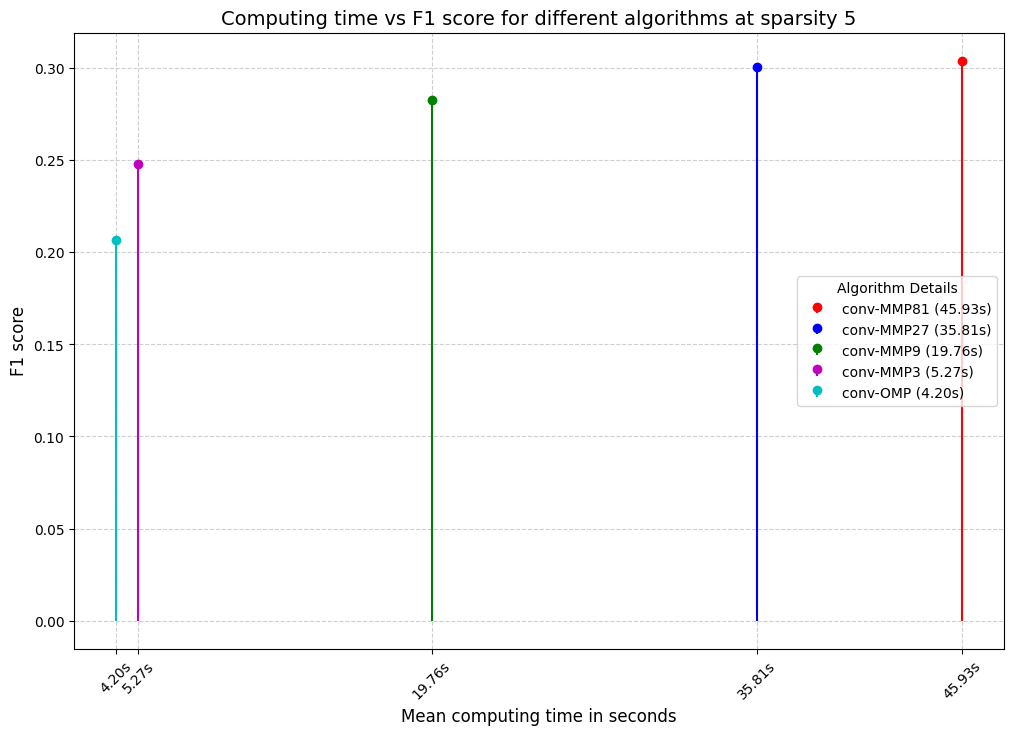
\includegraphics[width=1\linewidth]{images/trade_off_f1.png}
    \caption{Compromis entre la performance et le temps de calcul pour les algorithmes de déconvolution.}
    \label{fig:trade_off_f1}
\end{figure}    

\section{Conclusion}

En conclusion de ce stage, nos recherches ont contribuées à l'implémentation d'une nouvelle méthode de déconvolution parcimonieuse grâce à l'adaptation de l'algorithme Multipath Matching Pursuit (MMP) au contexte convolutionnel. 

Nous avons développé une méthode scalable plus précise que l'Orthogonal Matching Pursuit (OMP) pour les environnements critiques. Cela a conduit à une amélioration substantielle dans le traitement des motifs de défauts superposés.

Cette adaptation a non seulement amélioré la précision dans la détection et la caractérisation des défauts mais a aussi optimisé le compromis entre le temps de calcul et la performance. Les travaux menés ouvrent des perspectives pour des recherches futures dans des contextes critiques où la précision et la parcimonie des solutions sont nécessaires.

\section{Annexes}   

\subsection{Chronologie du stage effectué du 15 mai au 02 aout 2024}

\paragraph{Semaine du 20 mai}
Lecture des articles de référence et des travaux précédents sur le sujet \cite{orthogonal_matching_pursuit, localized_defects_omp, broken_wire}. Prise en main des outils de travail et des données disponibles. Début de l'implémentation de l'algorithme OMP avec des classes de base pour les atomes paramétrés et le dictionnaire : \texttt{ZSAtom}, \texttt{ZSDictionary}.

\paragraph{Semaine du 27 mai}
L'algorithme OMP fonctionne correctement et on constate quelqeus erreurs sur des signaux synthétiques un peu complexe. Utilisation de la fonction \texttt{oaconvolve} pour calculer la convolution à partir de la FFT. Implémentation d'une pipeline de calculs parallélisés avec \texttt{joblib} pour faire tourner l'OMP sur les serveurs distants en SSH.

\paragraph{Semaine du 3 juin}
Histogramme de l'erreur en position de l'OMP pour véririfier que l'erreur n'est pas biaisé.
Implémentation des algorithmes d'appariemment pour vérifier les performances de déconvolution.
Validation de l'OMP et lectures des articles qui proposent un raffinement de l'OMP \cite{swapping_based_refinement_omp, random_refined_omp, multipath_matching_pursuit}.

\paragraph{Semaine du 10 juin}
Après réflexions et réunion, décision de développer un algorithme de type \textit{multipath}.
Lecture de l'article \cite{triangle_inequalities} pour créer une heuristique pour éviter de calculer le vecteur des corrélations inter-atomiques.
Implémentation des classes \texttt{MMPNode} et \texttt{MMPTree} pour la construction récursive de l'arbre de recherche.
L'algorithme fonctionne correctement avec le mécanisme de réutilisation des noeuds calculés.

\paragraph{Semaine du 17 juin}
Début de la rédaction d'un article, implémentation des pipelines de génération de résultats pour les signaux synthétiques. Implémentation de la classe \texttt{CSCWorkbench} pour analyser des résultats.
Lancement des premières expériences avec le score F1.

\paragraph{Semaine du 24 juin}
Après réunion, décision de mettre en évidence la capacité de déconvolutio nsur des intervalles présentant plusieurs atomes superposés. 
Implémentation de l'expérience du boxplot pour mesurer l'erreur de reconstruction en fonction de la densité d'atomes superposés.
Rédaction d'une première version d'article à destination de la communauté informatique.

\paragraph{Semaine du 1 juillet}
Rédaction d'une nouvelle version de l'article pour la conférence ICASSP, International Conference on Acoustics, Speech, and Signal Processing, article court de 4 pages à destination d'une communauté traitement du signal.
Implémentation de méthode $\ell_1$ avec \texttt{SPORCO} en vain, on utilisera finalement la méthode \texttt{update\_z} du module \texttt{alphaCSC}.

\paragraph{Semaine du 8 juillet}
Tentative de construction d'une courbe ROC en vain car le contexte convolutionnel ne permet pas de définir une classe de faux positifs distinctes des faux négatifs. 
Implémentation de l'expérience de la courbe PRC : Precision-Recall Curve pour mesurer le compromis entre la précision et le rappel afin d'obtenir une métrique de comparaison avec les algorithmes basés sur la norme $\ell_1$.
Ce diagramme permet de se passer de la calbiration du facteur de régularisation $\lambda$ pour la méthode $\ell_1$. 

%\begin{figure}[H]
%    \centering
%    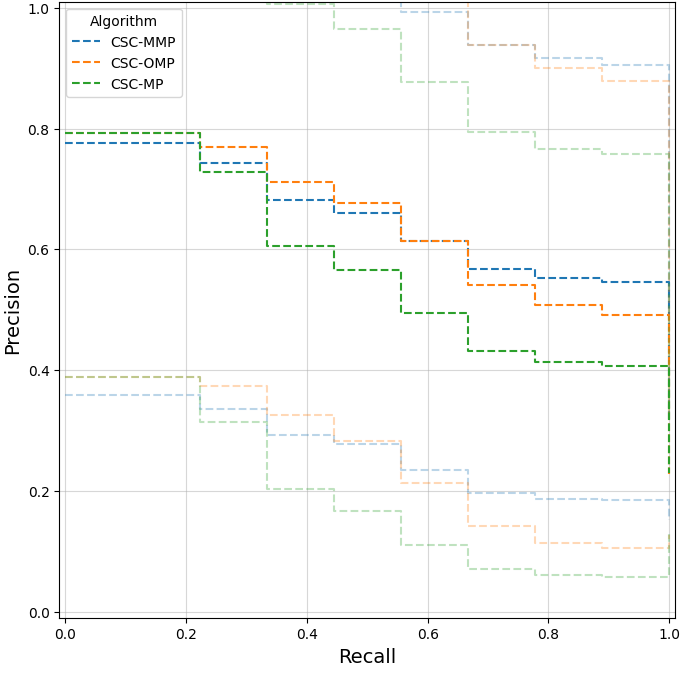
\includegraphics[width=0.6\linewidth]{images/prc2.png}
%    \caption{Courbe PRC pour mesurer le compromis entre la précision et le rappel.}
%    \label{fig:prc}
%\end{figure}

\paragraph{Semaine du 15 juillet}
Après beaucoup d'essais et de paramètres différents pour obtenir une PRC probante on décide de se tourner vers une métrique plus adaptée au contexte particulier de classification dans le cas convolutionnel à savoir le critical difference diagram.
Rédaction de l'article pour ICASSP.



\paragraph{Semaine du 22 juillet}
Implémentation du critical difference diagram pour mesurer la performance des algorithmes de déconvolution.
Rédaction de l'article pour ICASSP.

\paragraph{Semaine du 29 juillet}
Implémentation des expériences pour mesurer le compromis par rapport au temps de calcul.
Rédaction de l'article pour ICASSP.

\printbibliography

\begin{table}[H]
    \centering
    \caption{L'algorithme MMP-DF}
    \renewcommand{\arraystretch}{1.4} 
    \begin{tabular}{>{\arraybackslash}p{9cm}}
        \toprule
        \textbf{Entrée :} \\
        Mesure $\mathbf{y}$, matrice de capteurs $\boldsymbol{\Phi}$, parcimonie $K$, nombre d'expansion $L$, seuil d'arrêt $\epsilon$, nombre maximal de candidats de recherche $N_{\text{max}}$ \\
        \textbf{Sortie :} \\
        Indice de branche argmin MSE MMP-DF $\hat{\ell}$, atomes récupérés $\big\{\boldsymbol{\theta}_{\hat{\ell}}^k\big\}_{k \in \llbracket1, K\rrbracket}$, estimation de la reconstruction du signal $\hat{\mathbf{x}}$ \\
        \textbf{Initialisation :} \\
        $i:= 0$ (ordre des candidats), $\rho := \infty$ (magnitude minimale du résiduel) \\
        
        \midrule
        
        \textbf{tant que} $i < N_{\text{max}}$ \textbf{et} $\epsilon < \rho$ \textbf{faire} \\
    
        \quad $i := i + 1$ \\
        \quad $\mathbf{r}_{\ell}^0 := \mathbf{y}$ \\
        \quad $[c_1, \ldots, c_K] := \text{compute\_ck}(\ell, L)$ \hfill (calculer l'ordre des couches) \\
        
        \quad \textbf{pour} $k = 1$ \textbf{à} $K$ \textbf{faire} \\

        \quad \quad $\mathcal{J}_{\ell}^k = \underset{\mathcal{J} \in \llbracket 1, \widetilde{T}p \rrbracket^L}{\argmax} \Big\| \big( \boldsymbol{\Phi}^T  \mathbf{r}_{\ell}^k \big)_\mathcal{J} \Big\|_2^2 \text{ sous contrainte de } \mathcal{D}_\delta \big(  \big( \boldsymbol{\Phi} \big)_\mathcal{J} \big)$
        
        \quad \quad $\mathbf{S}_{\ell}^k := \mathbf{S}_{\ell}^{k-1} \cup \{\mathcal{J}_{\ell}^k [c_k]\}$ \hfill (construire un chemin dans la couche $k$-ième) \\
        \quad \quad $\hat{\mathbf{x}}_{\ell}^k := \boldsymbol{\Phi}_{\mathbf{S}_{\ell}^k}^\dagger \mathbf{y}$ \hfill (estimer $\hat{\mathbf{x}}_{\ell}^k$ dans la couche $k$-ième) \\
        \quad \quad $\mathbf{r}_{\ell}^k := \mathbf{y} - \boldsymbol{\Phi}_{\mathbf{S}_{\ell}^k} \hat{\mathbf{x}}^k$ \hfill (mettre à jour le résiduel) \\
        \quad \textbf{fin pour} \\
        
        \quad \textbf{si} $\|\mathbf{r}_{\ell}^k\| < \rho$ \textbf{alors} \hfill (mettre à jour le plus petit résiduel) \\
        \quad \quad $\rho := \|\mathbf{r}_{\ell}^k\|$ \\
        \quad \quad $\hat{\mathbf{x}} := \hat{\mathbf{x}}_{\ell}^k$ \\
        \quad \textbf{fin si} \\
        \textbf{fin tant que} \\
        \textbf{retourner} $\hat{\mathbf{x}}$ \\
        \midrule
        \textbf{fonction} compute\_ck($i, L$) \\
        \quad $temp := i -1 $ \\
        \quad \textbf{pour} $k=1$ \textbf{à} $K$ faire \\
        \quad \quad $c_k := \operatorname{mod}(temp, L) + 1$ \\
        \quad \quad $temp := \operatorname{floor}(temp/L)$ \\
        \quad \textbf{fin pour} \\
        \quad \textbf{retourner} $[c_1, \ldots, c_K]$ \\
        \textbf{fin fonction} \\
        \bottomrule
    \end{tabular}
    \label{table:mmp-df}
\end{table}

\end{document}